\documentclass[12pt,letterpaper]{article}
\usepackage[latin1]{inputenc}
\usepackage{amsmath}
\usepackage{amsfonts}
\usepackage{amssymb}
\usepackage{makeidx}
\usepackage{graphicx}
\usepackage[normalem]{ulem}
\usepackage{setspace}
\usepackage{subcaption}
\usepackage{float}
\usepackage{titlesec}
\usepackage[margin=1in]{geometry}
\usepackage{hyperref}
\usepackage{ntheorem}
\newtheorem{hyp}{Hypothesis}
\newtheorem{subhyp}{Hypothesis}[hyp]
\renewcommand\thesubhyp{\thehyp.\alph{subhyp}}
\usepackage[round]{natbib}
\bibpunct{(}{)}{;}{a}{}{,~}
\usepackage[space]{grffile}
\graphicspath{{./figures/}}
\usepackage[affil-it]{authblk}
\makeatletter
\def\@maketitle{%
	\newpage
	\null
	\vskip 2em%
	\begin{center}%
		\let \footnote \thanks
		{\Large\bfseries \@title \par}%
		\vskip 1.5em%
		{\normalsize
			\lineskip .5em%
			\begin{tabular}[t]{c}%
				\@author
			\end{tabular}\par}%
		\vskip 1em%
		{\normalsize \@date}%
	\end{center}%
	\par
	\vskip 1.5em}
\makeatother

\title{Friends Without Benefits: Explaining Costly Contributions to Unnecessary Wartime Coalitions}

\author{J Andr\'{e}s Gannon%
	\thanks{Electronic address: \texttt{jagannon@ucsd.edu}}}
\affil{Department of Political Science \\ University of California, San Diego}

\author{Daniel Kent%
	\thanks{Electronic address: \texttt{kent.249@osu.edu} \\ Acknowledgments. This research was sponsored by Office of Naval Research Grant N00014-14-1-0071 and the Department of Defense Minerva Research Initiative. Any opinions, findings, and conclusions or recommendations expressed in this publication are those of the authors and do not necessarily reflect the view of the Office of Naval Research.}}
\affil{Department of Political Science \\ Ohio State University}

\begin{document}
\maketitle

\begin{abstract}
What determines the magnitude of alliance contributions to conflict theaters? At the outbreak of the 1990 Persian Gulf War, the French military's budget was approximately double that of their Italian counterpart -- 58,149 and 30,768 million 2015 U.S. dollars, respectively.\footnote{\url{https://www.sipri.org/sites/default/files/Milex-constant-2015-USD.pdf}} However, in troops alone, France contributed over ten times as many forces to the conflict as Italy -- 20,000 as opposed to 1,900 military personnel. Though the Italian forces were not without value, their relative size demonstrates a simple but important point: not all alliance commitments are created equal. Indeed, if an ally is not expected to provide resources to a conflict in proportion with its capabilities, then the alliance itself is of far less consequence than it would otherwise be. Yet, empirical investigations of alliances and conflict processes tend
to avoid this distinction, instead focusing on: the formation of alliances, how alliances influence the initiation of disputes, or how alliances link to issues beyond the use of military force. We shed light on this important topic by developing a theoretical framework for and conducting an empirical investigation of the determinants of alliance contributions to conflict theaters. Through a new data set of country-level military portfolios and contributions to conflicts, we measure the type of technologies and amount of forces that states have deployed in conflict theaters since the end of the Cold War. We then apply techniques for statistical inference in social networks to produce insights into the strategic considerations that influence decisions to provide various military capabilities to ongoing conflicts. This project (something about how it will help the lit and is relevant to current debates about alliance reliability amidst various stresses to the international order -- NATO, North Korea, China.)
\end{abstract}

\section{Introduction}
	In 2001 the United States launched the war in Afghanistan with the goal of overthrowing the Taliban and dismantling Al Qaeda. But it did not do so alone; instead it led a coalition of 50 other states that fought alongside the United States until it formally ended in 2014. Not every state contributed equally. While the United States sent thousands of troops for the duration of the conflict, others contributed only a handful to fulfill their contractual alliance obligations under NATO. Yet some state had no formal alliance obligations and still sent troops in a manner that risked significant costs for that state. New Zealand lost almost a dozen troops in the Afghanistan conflict; a difficult thing for a state leader to justify to their public when the outcome of the conflict is largely immaterial to the state at hand.
	
	This is exemplary of a broader trend in coalition warfare. Some states contributes forces to coalition wars because they care about the material outcome of the conflict and hope to influence that outcome in some significant way. Others contribute forces because alliance obligations or expectations create a cost to free riding. But neither of those theories explain contributions like that of New Zealand to the war in Afghanistan; states that are unaffected by the outcome of the conflict, that have no notable ability to influence the outcome of the war, that experience no reputational cost from refusing to participate, and yet willingly risk high costs from their participation.
	
	This paper explains such contributions by developing a new theory about contributions to coalition warfare by states whose primary objective in fighting is not to influence the outcome of maintain their current reputation as reliable allies who fulfill their contractual obligations. We develop a new theory of states who contribute forces to coalition warfare in order to \textit{develop} their reputation as reliable allies because their contribution is disproportionally costly in terms of their baseline ability to contribute based on the size of their armed forces. We find that if state military contributions are measured not by the number of troops they contributed, but the proportion of their military forces they contributed, that states seeking to develop a stronger relation with the central actor in the coalition network are more likely to have higher proportional troop contributions. In other words, states that want to increase their ties to central actors in the coalition network do so by over-contributing a larger portion of their armed forces relative to states that were formally obligated to partake in coalition operations. This finding has important implications for understanding a costly means by which states seek to re-align themselves in international alliance networks. We think of conflict as a costly tool states employ to achieve their international objectives. One of those objectives is unrelated to the outcome of the conflict and instead relies on using war efforts to signal to other states that you are willing to undergo a large cost to help them achieve their goal with the hopes that this will improve your relationship with them in the future. This can help explain ways that states use unnecessary wars to gain the attention and (hopefully) respect of central players in the international system. War can be a good excuse for improving your ties with important states.
	
	This paper proceeds in five parts. In part two we explore existing explanations for coalition warfare that have thus far focused on the manner in which states fight together rather than explaining why they bother fighting together at all. Part three develops our theory by applying the costly signaling theory to coalition warfare using a innovative measure of the costliness of a state's contribution to coalition warfare; the relative pressure of that mobilization based on the size of its available armed forces. Part four empirically tests this finding by examining coalition contributions during the war in Afghanistan (2001-2014) which presents a ripe test case for our theory given variation in the alliance obligations of the states that participated as well as their level of participation. In section five we discuss the results of this empirical test and its generalizability for the broader theory explaining how states seek to alter their position within the network of capable international actors. Section six concludes.

\section{Existing Studies on Coalition Warfare}
	Why do countries fight together in coalitions
	
	Those that want to win
	
	Formal obligation from alliance conditions
	
	Assumes countries that fight together are already predisposed to have aligned interests. Doesn't look at how fighting together can alter the alignment of interests.
	
	Some work has looked at related areas like UN peacekeeping, we apply it in a different context where its easier to separate formal obligation from wanting to signal closer friendships, its easier to identify the central actor, and the costs are higher

\section{Theory of Signaling via Coalition Contributions}
	Nature of military contribution to conflict theater is predicted by a nation?s location in security community because that determines its primary international objective
	
	Central vs peripheral
		\begin{figure}[H]
			\centering
			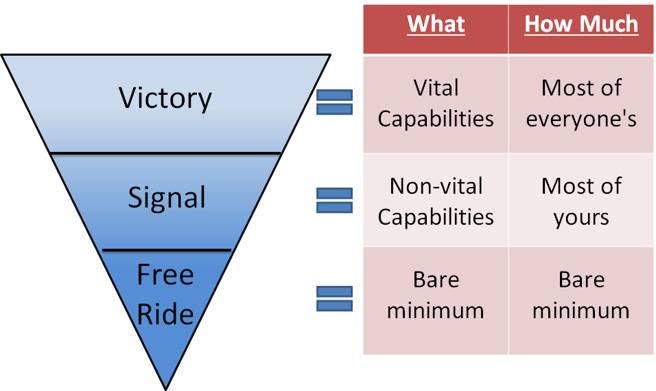
\includegraphics[width=0.6\textwidth]{contribution_pyramid.png}
			\caption{Theory of Coalition Warfare Contributions}
			\label{fig:theory}
		\end{figure}			

\section{Research Design}
	Unit of analysis: State (2001-2005)
	
	DV: Percent of national military personnel fighting in Afghanistan War
	
	EV: Preference Alignment with US/UK + Military pact with US/UK
	Controls: Military Pact, Ideal Point Distance from US,  Eigenvector Centrality in Preference Network, CINC score, Distance from Afghanistan
	
	Model: pact + ideal point + pact*ideal point + eigen + cinc + log(distance)

\section{Results}
	There is some empirical evidence that this had a positive outcome for New Zealand. They now participate in more joint military training exercises with NATO. ``...good opportunity for the New Zealand Defence Force to test its interoperability with contributing NATO nations. This deployment is an example of New Zealand's commitment to playing our part in supporting NATO in areas of common interest." -- Jonathan Coleman, New Zealand Defence Minister (2014)

\section{Conclusion}
	Takeaway -- Small states fight for future military cooperation
	Contribution -- New data on relative contributions helps explain free-riding exceptions
	Future work -- Does this payoff? Look at other coalition wars
	
	``In the Libya operation, Norway and Denmark, have provided 12 percent of allied strike aircraft yet have struck about one third of the targets...These countries have, with their constrained resources, found ways to do the training, buy the equipment, and field the platforms necessary to make a credible military contribution." -- US Defence Secretary Robert Gates (June 2011)

\bibliographystyle{apsr}
\bibliography{isaf_alliances.bib}

\end{document}
